%%%%%%%%%%%%%%%%%%%%%%%%%%%%%%%%%%%%%%%%%%%%%%%%%%%%%%%%%%%%%%%%%%
%%%%%%%% ICML 2016 EXAMPLE LATEX SUBMISSION FILE %%%%%%%%%%%%%%%%%
%%%%%%%%%%%%%%%%%%%%%%%%%%%%%%%%%%%%%%%%%%%%%%%%%%%%%%%%%%%%%%%%%%

% Use the following line _only_ if you're still using LaTeX 2.09.
%\documentstyle[icml2016,epsf,natbib]{article}
% If you rely on Latex2e packages, like most moden people use this:
\documentclass{article}

% use Times
\usepackage{times}
% For figures
\usepackage{graphicx} % more modern
%\usepackage{epsfig} % less modern
\usepackage{subfigure} 

% For citations
\usepackage{natbib}

% For algorithms
\usepackage{algorithm}
\usepackage{algorithmic}

% As of 2011, we use the hyperref package to produce hyperlinks in the
% resulting PDF.  If this breaks your system, please commend out the
% following usepackage line and replace \usepackage{icml2016} with
% \usepackage[nohyperref]{icml2016} above.
\usepackage{hyperref}

% Packages hyperref and algorithmic misbehave sometimes.  We can fix
% this with the following command.
\newcommand{\theHalgorithm}{\arabic{algorithm}}

% Employ the following version of the ``usepackage'' statement for
% submitting the draft version of the paper for review.  This will set
% the note in the first column to ``Under review.  Do not distribute.''
\usepackage{icml2016}

% Employ this version of the ``usepackage'' statement after the paper has
% been accepted, when creating the final version.  This will set the
% note in the first column to ``Proceedings of the...''
% \usepackage[accepted]{icml2016}

\usepackage{multirow}
\usepackage{amsmath,amsfonts,amsthm}
\usepackage{amssymb}

\DeclareMathOperator*{\argmin}{arg\,min}
\DeclareMathOperator{\prox}{prox}
\DeclareMathOperator{\Id}{Id}

\newcommand{\R}{\mathbb{R}}


% The \icmltitle you define below is probably too long as a header.
% Therefore, a short form for the running title is supplied here:
\icmltitlerunning{Informing High-Dimensional Inference in Neuroimaging}

\begin{document} 

\twocolumn[
\icmltitle{Hierarchical Region-Network Sparsity for\\
High-Dimensional Inference in Brain Imaging}
% \icmltitle{Region-Network Hierarchical Sparsity Priors for\\
% High-Dimensional Inference in Brain Imaging}

% It is OKAY to include author information, even for blind
% submissions: the style file will automatically remove it for you
% unless you've provided the [accepted] option to the icml2016
% package.
\icmlauthor{Danilo Bzdok}{danilo.bzdok@inria.fr}
\icmladdress{Department of Psychiatry, Psychotherapy and Psychosomatics, RWTH Aachen, Germany\\
  Parietal, INRIA, NeuroSpin, bat 145, CEA, 91191 Gif-sur-Yvette France}
\icmlauthor{Michael Eickenberg}{Michael.Eickenberg@normalesup.org}
\icmladdress{Department d'Informatique, Ecole Normale Superieure, Paris}
\icmlauthor{Ga\"el Varoquaux}{gael.varoquaux@inria.fr}
\icmlauthor{Bertrand Thirion}{bertrand.thirion@inria.fr}
\icmladdress{Parietal, INRIA, NeuroSpin, bat 145, CEA, 91191 Gif-sur-Yvette France}

% You may provide any keywords that you 
% find helpful for describing your paper; these are used to populate 
% the "keywords" metadata in the PDF but will not be shown in the document
\icmlkeywords{Sparsity-inducing norms, hierarchical tree sparsity,
numerical optimization,
systems neuroscience,
functional specialization, functional integration}

\vskip 0.3in
]

\begin{abstract} 
Structured sparsity penalization has recently improved
statistical models applied to high-dimensional data in various domains.
%
As an extension to imaging neuroscience,
the present work incorporates
priors on network hierarchies of brain regions into
logistic-regression to distinguish neural activity.
This recombines neurobiological architectures underlying
functional segregation into brain regions and
functional integration by brain networks
that are studied separately in neuroscientific research.
%
Hierarchical region-network priors are shown to better classify
18 psychological tasks from a reference dataset
than other sparse estimators.
Weighing the relative importance of
region and network structure within the hierarchical tree penalty
recovered complementary aspects of the neural activity patterns.
%
Local and global priors of neurobiological knowledge
are thus demonstrated to enhance
generalization performance, sample complexity, and domain interpretability.



\end{abstract} 

\section{Introduction}
% sparsity
Many quantitative scientific domains underwent a
recent passage from the classical regime (i.e., ``long data")  to
the high-dimensional regime (i.e., ``wide data").
% the high-dimensional regime (i.e., ``wide data") \cite{jordan2015massive}.
Also in the brain imaging domain,
many contemporary methods for acquiring brain signals yield
more variables per observation than
total observations per data sample.
This $n \ll p$ scenario challenges various statistical methods from
classical statistics.
For instance,
estimating generalized linear models without additional assumptions
yields an underdetermined system of equations.
%
Many such ill-posed estimation problems
have benefited from
\textit{sparsity} assumptions
\cite{hastie2015statistical}.
They act as a 
regularizer and can be used for model selection.
Sparse supervised and unsupervised
learning algorithms have proven to yield
statistical relationships that can be readily
estimated, reproduced, and interpreted
\cite{giraud2014introduction}.
%
Generally, \textit{structured sparsity} can impose
domain knowledge on the 
statistical estimation,
thus shrinking and selecting variables guided by
expected data distributions
\cite{bach2012optimization}.
Such restrictions to statistical complexity
are an attractive plan of attack
for the $\textgreater$100,000 variables per brain map.
Yet, what generally accepted neurobiological structure lends itself
to exploitation using structured sparsity priors?



% specialization & integration
Concepts on human brain organization have long been torn
between the two extremes
\textit{functional specialization} and \textit{functional integration}.
Functional specialization emphasizes that microscopically distinguishable
brain regions are responsible for distinct classes of computational 
processes
\cite{kanwisher2010functional}.
Conversely, functional integration emphasizes that brain function
is enabled by a complex interplay between these
distinct brain regions \cite{sporns14nn}.
%
Local
infrastructure
and unique global connectivity profiles are thought to go hand-in-hand
to realize brain function.
%
However,
probably no existing brain analysis method acknowledges that
both functional design principles are inextricably involved
in the realization of mental operations.



Functional specialization has long been
explored and interpreted based on different research methods.
%
For instance,
single-cell recordings and microscopic examination
revealed the
segregation of the occipital visual cortex into V1, V2, V3, V3A/B, and V4
regions
\cite{hubel1962receptive, zeki1978functional}.
Tissue lesion of the mid-fusiform gyrus of the visual system,
in turn,
was frequently reported to impair
recognition of others' identity from faces
\cite{iaria2008contrib}.
%
As a crucial common point,
all these methodological approaches
yield neuroscientific findings
that are naturally interpreted according to
non-overlapping, discrete region compartments
as the basic architecture of brain organization.
% INTEGRAL
It is more recent
that the main interpretational focus has shifted
from circumscribed regions to network stratifications
in systems neuroscience \cite{yuste2015}.
%
Besides analyses of
electrophysiological oscillations
% \cite{buzsaki2004neuronal}
and
graph-theoretical properties,
% graph-theoretical properties \cite{bullmore2009complex},
studies of
functional connectivity correlation \cite{buckner2013opportunities} and
independent component analysis (ICA) \cite{beckmann2005}
became the workhorses of network discovery
in neuroimaging.
%
As a common point of this second set of methods,
interpretation of findings naturally embraces
cross-regional integration by
overlapping network compartments
as the basic architecture of brain organization,
in stark constrast to methods examining regional specialization.


% % specialization & integration
% Concepts on human brain organization have long been torn
% between the two extremes
% \textit{functional specialization} and \textit{functional integration}.
% Functional specialization emphasizes that microscopically distinguishable
% brain regions are responsible for distinct classes of computational 
% processes
% \cite{kanwisher2010functional}.
% Functional integration, in turn, emphasizes that brain function
% is enabled by complex connections between these
% distinct brain regions \cite{sporns14nn}.
% %
% These notions were predominantly derived from
% invasive examination of anatomy (i.e., histological preparation),
% connectivity (i.e., axonal tracing),
% and functional properties
% (i.e., single-cell recordings) in animals.
% Regarding functional segregation into specialized regions,
% early histological investigations into the microscopic heterogeneity of
% the human cerebral cortex have resulted
% in several detailed anatomical maps
% \cite{brodmann1909vergleichende}.
% Regarding axonal connections,
% each such cortical area has been observed
% to possess a unique set of incoming and outgoing connections
% \cite{passingham2002, young93monkey, scannell95cat}.
% %
% Both
% local
% %cyto- and chemoarchitectonic
% infrastructure
% and its unique global connectivity profile
% together are thought to realize brain function.
% %
% In sum,
% cortical brain modules versus connections between them
% reflect 
% functional specialization versus functional integration
% \cite{friston2002beyond, mesulam_sensation}.
% Importantly,
% probably no existing brain analysis method acknowledges that
% both functional organizations are inextricably involved
% in the realization of mental operations
% \cite{tononi1998complexity, saygin2012}.
% 
% 
% 
% % SPECIAL
% Functional specialization has been
% explored and interpreted based on many different research methods.
% %
% Single-cell recordings and microscopic examination
% revealed, for instance, the
% specialization in the occipital visual cortex into V1, V2, V3, V3A/B, and V4
% \cite{hubel1962receptive, zeki1978functional}.
% Tissue lesion of the mid-fusiform gyrus of the visual system,
% in turn,
% was frequently reported to impair
% recognition of others' identity from faces
% \cite{iaria2008contrib}.
% The whole-brain localization of
% sensory, motor, and emotional functions to cortical areas
% % in the living brain
% was later enabled by
% non-invasive brain imaging with
% functional magnetic resonance imaging (fMRI) and
% positron emission tomography (PET)
% \cite{fristen1997imaging}.
% Further,
% radioactive mapping of neurotransmitter receptors
% rendered accessible yet another
% local characteristic of neuronal populations
% \cite{zilles2009receptor}.
% % allude to our many-regions layer in our methods
% In the computational era,
% automatic clustering methods are increasingly employed to
% regionally differentiate the cerebral cortex,
% which can partly be more fine-grained than
% classical microscopical borders
% \cite{behrens03, cbp2015review}.
% High-thoughput approaches today enable
% ultrahigh-resolution 3D models of brain anatomy
% at near-cellular scale
% \cite{amunts2013bigbrain}.
% %
% As a crucial common point,
% all these methodological approaches
% yield neuroscientific findings
% that are naturally interpreted according to
% non-overlapping, discrete region compartments
% as the basic architecture of brain organization.
% 
% 
% 
% % INTEGRAL
% It is more recent
% that the main interpretational focus has shifted
% from circumscribed regions to network stratifications
% in systems neuroscience \cite{yuste2015, stephan_dys}.
% %
% Invasive axonal tracing studies in monkeys were complemented
% by diffusion MRI tractography in humans
% as a now frequently employed method to
% outline fiber bundles between brain regions
% \cite{jbabdi2013long}.
% Besides analyses of
% electrophysiological oscillations
% \cite{buzsaki2004neuronal}
% and
% graph-theoretical properties \cite{bullmore2009complex},
% studies of
% functional connectivity \cite{buckner2013opportunities} and
% independent component analysis (ICA) \cite{beckmann2005}
% became the workhorses of network discovery
% in neuroimaging.
% These revealed the important implication of
% canonical brain networks across psychological tasks,
% including the so-called
% ``default-mode network'' \cite{raichle2001pnas},
% ``salience network'' \cite{seeley2007dissociable},
% and ``dorsal attention network'' \cite{corbettashul2008}. 
% Characteristic changes in the configuration of
% these macroscopical networks
% were repeatedly observed to be induced
% by the onset of given psychological tasks \cite{fransson2006}.
% % Such task-induced mechanisms orchestrating supraordinate networks
% % might be subserved by the right anterior insula \cite{sridh2008}
% % and temporo-parietal junction \cite{bzdok2013tpj}.
% %
% As a common point of all these methods,
% interpretation of findings naturally embraces
% cross-regional integration by
% overlapping network compartments
% as the basic architecture of brain organization,
% in stark constrast to methods examining regional specialization.



% study
Building on these two major interpretational traditions in neuroscience,
the present study proposes to incorporate
established neurobiological structure underlying
functional segregation and integration
into supervised estimators
by hierarchical structured sparsity.
% The "true" relative importance of 
% local region compartments and global network compartments
% is typically unknown
% but
% probably varying in degree
% across diverse neuroscientific questions.
%
Learning algorithms
exploiting structured sparsity 
have recently made much progress in various domains
from processing auditory signals \cite{daudet2004sparse},
natural images \cite{harzallah2009combining} and
videos \cite{kang2015structured}
% videos \cite{kang2015structured, kim2010sparse}
to
astrophysics \cite{vinci2014estimating},
genetics \cite{kim2012tree},
% genetics \cite{rapaport2008classification, kim2012tree},
and
conformational dynamics of protein complexes \cite{jenatton2009structured}.
%
The hierarchical tree penalties recently suggested for imaging neuroscience
\cite{jenatton2011multi} will be extended
by introducing neurobiologically plausible region and network priors
to design neuroscience-specific estimators.
%
Based on the largest public neuroimaging repository
(Human Connectome Project [HCP], \url{http://www.humanconnectomeproject.org/}),
we demonstrated that domain-informed supervised models
gracefully tackle the curse of dimensionality,
yield more human-interpretable results,
and generalize better to new samples
than domain-naive estimators.

\section{Methods}
The main contribution is the domain adaptation of hierarchical structured
tree penalties to jointly incorporate region 
specialization and network integration priors into multivariate 
estimators.
We capitalize on hierarchical group lasso as recently introduced
\cite{jenatton2011multi} to create a set of convex penalty terms.
These allow acknowledging the interplay between local specialization and 
global connectivity when discriminating defined psychological tasks
from brain activity.
% Bertrand: univariate-multivariate is orthogonal to the
% current study -> make clear why we opted for multivariate
% rather than univariate which might even have been simpler
Rather than inferring brain activity from psychological tasks
in a univariate setting,
this study infers psychological tasks from brain activity
in a multivariate setting to allow for
prediction in unseen neuroimaging data.
%
\subsection{Rationale}
% \paragraph{Rationale.}
3D brain maps obtained by neuroimaging
techniques are high-dimensional but, luckily,
their signal is highly structured.
Its explicit dimensionality, the number of brain voxels,
typically exceeds 100,000 variables, while the number
of samples rarely exceeds few hundreds.
This $n \ll p$ scenario directly implies underdetermination of any
linear model based on dot products with the voxel values.
However, the effective dimensionality of functional neuroimaging data has been
shown to be much lower \cite{bzdok2015semi}.
Two types of low-dimensional neighborhoods will be exploited by
injecting established knowledge of regional specialization
(i.e., region priors)
and spatiotemporal interactions
(i.e., network priors)
into the statistical estimation process.



Large-scale brain networks emerge in human individuals around birth
\cite{doria2010}, before mental capacities mature in childhood. 
In adults,
the sets of regions that compose
a given spatiotemporally cohesive network are known to have more
similar functional profiles than nodes from different networks
\cite{anderson2013}.
As a well-established method for network estimation
\cite{beckmann2005},
ICA yields continuous brain maps with
weights for each voxel. The region nodes of ICA
networks are spatially disjoint sets of voxel groups that
agree with boundaries of brain atlases.
Such brain atlases can be obtained by segregating
the brain's grey matter into spatially compact voxel groups
using clustering algorithmisms
\cite{cbp2015review}.
Consequently,
each region from a brain atlas can be uniquely associated with one
the extracted ICA networks.
%
In the present work previously published network definitions
obtained using ICA \cite{smith2009}
and
previously published region definitions obtained from
spatially constrained ward clustering \cite{crad12}
allow constructing a hierarchy of global ICA networks with their
assigned local cluster regions.
The ensuing network-region tree is used as a structural prior
of expected weight distributions
during supervised model fitting.



This tree structure can be seamlessly plugged into
a recently introduced hierarchical sparsity estimator
\cite{jenatton2011multi}.
It extends the group lasso
\cite{yuan2006model}
by permitting variable groups that contain each other
in a nested tree structure.
The first hierarchical level of that tree are
the network groups that contain all
the voxels of the brain regions associated to them.
Each network node, in turn, descends into a second hierarchical level of
brain regions of spatially neighboring voxel groups.
%
As a consequence of such a region-network sparsity tree,
a child node enters the set of relevant voxel variables only
if its parent node has been selected
\cite{bach2012optimization}.
Conversely,
if a parent node is deselected,
also the voxel variables of all child nodes are deselected.
%
Moreover,
the coefficient of all region groups and all network groups can
be weighed individually.
Trading off the voxel penalties of the network level against the
voxel penalties of the region level,
we can design different estimation regimes.
%
Setting a low penalty on the network groups makes it probable
that all of them are active in the estimated weight map. If we then select
higher penalties on region groups, selection of relevant region groups is
forced without negligable bias of the network definitions.
Conversely, setting low penalties on the region definitions
makes it possible for
all voxels to be active. Selecting higher penalties on the networks then
leads to a selection of networks with all regions associated to it.
%
This region-network tradeoff allows inspecting the relative contributions
of the region and network levels
of the hierarchical tree prior.


% \paragraph{Problem formulation.}
\subsection{Problem formulation}
We formulate our estimation problem in the framework of regularized risk
estimation applied to linear models: 
The goal is to estimate a good predictor of cognitive task
given a brain image. Let the set \(\mathcal X\subset\R^p\) represent brain
images of \(p > 0\) voxels.
%
We minimize the risk \(\mathcal L(\hat y, y)\) with
\(\hat y = f(X\hat w + \hat b)\), where \(f\) is a link function 
(e.g. sigmoid for logistic regression, identity for linear regression),
and \(\mathcal L\) usually represents an appropriate negative loglikelihood.
We incorporate a useful prior through regularization:
\[\argmin_{w, b} \mathcal L(f(Xw + b), y) + \lambda\Omega(w),\]
where \(\lambda > 0\) and \(\Omega\) is the regularizer.

Brain \textit{regions} are defined as disjoint groups of voxels. Let \(\mathcal G\)
be a partition of \(\{1, \dots, p\}\), i.e.
\[  \bigcup_{i} g_i = \{1, \dots, p\} \textrm{ and } g_i\cap g_j=\emptyset
\quad\forall i\not=j\]

Brain \textit{networks} consist of a group of one or several brain regions.
The set of brain networks \(\mathcal{H}\) also forms a partition of 
\(\{1, \dots, p\}\) and in addition it is consistent with \(\mathcal G\) in
the sense that
\[\textrm{for all }g\in\mathcal G, h\in\mathcal H,\quad
\textrm{ either } g\subset h\textrm{ or }g\cap h = \emptyset.\]
This allows the association of each region \(g\in\mathcal G\) to a 
network \(h\in\mathcal H\) and thus establishes a tree structure (up to 
adding a root node containing all voxels).

For a brain image \(w\in\R^p\) and a group \(g\), the vector 
\(w_g\in\R^{|g|}\) is defined as the restriction of \(w\) to the coordinates
 in \(g\). The structured penalty incorporating network
and region information can then be written as
\[\Omega(w) = \alpha\sum_{h\in\mathcal H}\eta_h\|w_h\|_2 + \beta\sum_{g\in\mathcal G}\eta_g\|w_g\|_2.\]
According to \cite{yuan2006model} we set \(\eta_g = 1/\sqrt{|g|}\) to
account for varying group size. The hierarchy-level-specific factors 
\(\alpha > 0\) and \(\beta > 0\) are used to trade-off region-weighted and
network-weighted models against each other.

One can read off the formula that decreasing \(\alpha\) leads to less 
penalization of brain networks and thus to tendentially fully active groups
and dense brain maps. If at the same time \(\beta\) is increased to 
induce group sparsity, then only the structure of brain regions encoded
by \(\mathcal G\) is present. Conversely, if \(\beta\) is chosen 
sufficiently small, and \(\alpha\) increased,
then the structure will come from \(\mathcal H\), leading to the
selection of brain networks rather than regions.

It is important to note that the above trade-off shows that predominance
can be either attributed to regions or networks, but that nevertheless the
penalty structure is hierarchical: If the network penalty layer sets a
network group to zero, then all the contained region groups are forced to
have activity zero. Conversely, if a brain region has non-zero coefficients,
then necessarily the network containing it must be active.
This relation is asymmetric, the roles of \(\mathcal G\) and \(\mathcal H\) 
cannot be swapped: A brain 
region can set all its coefficients to zero without forcing the 
corresponding network to zero. A brain network can be active without its
subregions being active.
When evaluating the trade-off in \((\alpha, \beta)\), this needs to be taken
into account.

The prediction problem at hand is a multiclass classification. We choose to
attack this using one-vs-rest scheme on a binary logistic regression, whose
loss can be written as
\[\sum_{i=1}^n\log(1 + \exp(-y_i\langle x_i, w\rangle)) + \lambda\Omega(w),\]
if \(y\in\{-1, 1\}\) and with \(x_i\in\R^p\) the training sample brain images.
We optimize parameters \(w\) using an iterative forward-backward
scheme analogous to FISTA for the lasso \cite{beck2009}.

% \paragraph{Optimization.}
% We optimize the data loss function using an iterative forward-backward
% scheme analogous to FISTA for the lasso \cite{beck2009}. 
% We divide the
% loss \(\mathcal L(w)\) into a smooth, convex data fit term \(F(w)\) (here: 
% logistic regression loss) and a potentially non-smooth, convex 
% regularization term \(G(w)\). 
% Define \(\prox_{\gamma G}(v) = (\Id + \gamma\partial G)^{-1}(v)\), where \(\partial G\) is the subdifferential of \(G\) and 
% let \(\nabla F(v)\) be the gradient of \(F\) in \(v\). Further let \(L > 0\)
% be a Lipschitz constant of the gradient of \(F\) and choose a step size
% \(\varepsilon\in (0, \frac{2}{L})\). Starting with an arbitrary 
% initialization of \(w_0\), putting \(z_1 = w_0\) and \(t_1 = 1\), then for
% \(k\geq 1\) until convergence do:
% \begin{eqnarray*}
%   x_k & = & \prox_{\varepsilon G}(y_k - \varepsilon\nabla F(y_k))\\
%   t_{k + 1} & = & \frac{1 + \sqrt{1 + 4 t_k^2}}{2}\\
%   y_{k + 1} & = & x_k + \left(\frac{t_k - 1}{t_{k + 1}}\right)(x_k - x_{k - 1})
% \end{eqnarray*}
% In our case \(G(v) = \lambda\Omega(v)\). Splitting \(\Omega(v) = \Omega_{\mathcal H}(v) + \Omega_{\mathcal G}(v)\) with 
% \(\Omega_{\mathcal H}(v) = \alpha\sum_{h\in\mathcal H}\eta_h\|v_h\|_2\) and
% \(\Omega_{\mathcal G}(v) = \beta\sum_{g\in\mathcal G}\eta_g\|v_g\|_2\), we observe
% that \[\prox_{\varepsilon\lambda\Omega_{\mathcal H}}(v) = \sum_{h\in\mathcal H}\iota_h\left([\|v_h\|_2 > \eta_h\varepsilon\lambda\alpha]\left(v_h - \eta_h\varepsilon\lambda\alpha\frac{v_h}{\|v_h\|_2}\right)\right),\]
% where \(\iota_h\) is the canonical injection of the group \(h\) into 
% \(\R^p\) (if \(\pi_g: v\mapsto v_g\), then \(\iota_g = \pi_g^\ast\) the 
% adjoint/transposed operator). This holds analogously for 
% \(\Omega_{\mathcal G}\).
% According to \cite{jenatton2011}, the proximal operator of 
% the hierarchical penalty \(\varepsilon\lambda\Omega\) is
% \[\prox_{\varepsilon\lambda\Omega}(v) = \prox_{\varepsilon\lambda\Omega_{\mathcal H}}\circ\prox_{\varepsilon\lambda\Omega_{\mathcal G}}(v).\]



% \paragraph{Hyperparameter optimization.}
\subsection{Hyperparameter optimization}
The stratified and shuffled training data were submitted
to a nested cross-validation scheme
for model selection and model assessment.
In the inner CV layer, the logistic regression estimators
have been trained in a one-versus-rest design that
distinguishes each class from
the respective 17 other classes
(number of maximal iterations=$100$, tolerance=$0.001$).
{\color{red} In the outer CV layer, grid search
selected among candidates for the respective $\lambda$ parameter
by searching between $10^{-2}$ and $10^{1}$ in 9 steps on a logarithmic scale.}
Importantly, the thus selected sparse logistic regression classifier was
evaluated on an identical test set in all settings.



%% Sparse linear models
%% encode geometric prior information
%% topology
%% local sets of voxels
%% 
%% Group-sparsity is a first step towards the more general idea that
%% a regularization function can encourage sparse solutions with a particular structure. 
%% 
%% it is not realistic to assume that all of the tasks share the same set of rele- vant inputs as in the L1/L2-regularized regression. A subset of highly related outputs may share a common set of relevant inputs, whereas weakly related outputs are less likely to be affected by the same inputs.
%% 
%% structured regularization
%% We might therefore gain in the quality of the factors
%% induced by enforcing directly this a priori 
%% 
%% groups at multiple granularity
%% 
%% tree-guided group lasso
%% 
%% encourage structured shrinkage effect 
%% 
%% l1 = unstructured sparsity-inducing penalty
%% 
%% Our method extends the L1/L2 penalty to the tree-lasso penalty
%% by letting the hierarchically-defined groups overlap. 
%% the tree lasso is a special case of overlapping group lasso
%% 
%% for every column u of U, it compute a column v of V solving
%% 
%% we aim at learning a weight vector w ∈ Rp and an intercept b ∈ R
%% such that the prediction of y can be based on the value of w⊤x + b.
%% 
%% We omit a bias term, since the data were mean-centered
%% and unit-variance scaled.
%% The scalar b is not particularly informative
%% 
%% however the vector w corresponds to a volume that
%% can be represented in brain space as a volume
%% 
%% hierarchial tree = more generally into a directed acyclic graph
%% 
%% more precisely, we denote by X ∈ Rn×p the design matrix
%% assembled from n fMRI volumes and by y ∈ Rn the corresponding n targets.
%% In other words, each row of X is a p-dimensional sample,
%% i.e., an activation map of p voxels related to one stimulus presentation.
%% for visualization of the predictive pattern of voxels. 
%% 
%% Learning the parameters (w, b) remains challenging
%% since the number of features (104 to 105 voxels) exceeds
%% by far the number of samples (a few hundreds of volumes). 
%% 
%% The scalar b is not particularly informative,
%% however the vector w corresponds to a volume that
%% can be represented in brain space as a volume
%% for visualization of the predictive pattern of voxels.
%% 
%% each row of X is a p-dimensional sample,
%% i.e., an activation map of p voxels related to one stimulus presentation.
%% 
%% To address this issue, dimensionality reduction attempts to
%% find a low dimensional subspace that concentrates
%% as much of the predictive power of
%% the original set as possible for the problem at hand.
%% -> we do not want to do preliminary feature selection or
%% dimensionality reduction
%% or feature agglomeration because we want to fit one model parameter
%% to each brain voxel for maximal interpretability
%% This corresponds to discarding some columns of X.
%% 
%% The essential shortcoming of the Elastic net is that
%% it does not take into account the spatial structure of the data,
%% which is crucial in this context
%% 
%% Craddock clusters are often used for feature agglomeration
%% into parcels
%% -> exploits only a part of the data
%% 
%% dual-level spatial structure
%% sparse hierarchical regularization
%% structured sparsity-inducing regularization
%% the root of the tree T is the unique cluster that gathers all the voxels,
%% 
%% It is a generalization of the traditional $\ell_1$-norm
%% $\Omega(\mathbf{w}) = \sum_{j=1}^p|\mathbf{w}_j|$
%% ignores structure
%% 
%% 
%% \cite{jenatton2011multi}
%% 
%% \textit{structured sparsity}
%% 
%% \cite{huang2011learning, morales2010family, jenatton2011structured}
%% 
%% 
%% a node $j$ of $\mathcal{T}$,
%% we denote by $g_j \subseteq \{1,..,q\}$ the set of indices that record
%% all the descendants of $j$ in $\mathcal{T}$
%% 
%% the family of sparsity-inducing norms has recently been extended
%% by hierarchical sparsity penalty terms
%% \cite{zhao2009composite}.
%% 
%% 
%% \begin{equation}
%%   \Omega(\mathbf{w}) = \sum_{g \in G}||\mathbf{w}_g||_2 = \sum_{g \in G}\sqrt{\sum_{j \in g}\mathbf{w}_j^2}
%% \end{equation}
%% 
%% For example, when G is the set of all singletons, Ω is the
%% usual l1 norm (assuming that all the weights are equal to 1).
%% 
%% l1/l2 mixed norm is convex
%% 
%% 
%% Discarding coefficients belonging to a network group will naturally enforce
%% discarding the coefficients belonging to each of its descendent region groups.
%% Conversely,
%% variable selection of a network group will also enforce
%% selection of all voxel of its descendent group regions.
%% Single region groups can however be set to zero (unselected)
%% or non-zero (selected)
%% without analogous effect on the parent network group.
%% 
%% 
%% 
%% 
%% At the between-group level,...
%% $\Omega$ exerts $\ell_1$-like variable selection on
%% the $(||\mathbf{w}_g||_2)_{g\in G}$ groups,
%% yielding a maximum of $g \in G$ to be zeroed out
%% \cite{jenatton2011structured}.
%% The important consequence is that also all descentes of such a zeroed
%% group $g \in G$ will be descarded.
%% Conversely,
%% if one group $g$ is selected,
%% then all the ancestral groups will also be selected.
%% Thus, statistical estimation will be improved by enticing
%% entire voxel sets to be selected or discarded as predictive, 
%% although one individual coefficient is computed for each voxel.
%% 
%% -> it is a $(\ell_1, \ell_2)$-mixed norm
%% -> between-group sparsity effect by l1
%% -> within-group shrinkage effect by l2
%% 
%% 
%% \begin{equation}
%%   \Omega(\mathbf{w}) = \sum_{g \in G} \eta_g ||\mathbf{w}_g||_2
%% \end{equation}
%% 
%% $(\eta_g)_{g \in G}$ are positive weights for the groups
%% 
%% 
%% fit to the data is measured through
%% a convex loss function (w, b) 􏰀→ L(y, X, w, b) ∈ R+. 
%% 
%% 
%% \paragraph{Classification}
%% 
%% logistic loss function
%% 
%% \begin{equation}
%%   P(y=k|x, W, b) = \frac{exp\{x^Tw^k + b_k\}}{\sum_{m=1}^cexp\{x^Tw^m + b_m\}}
%%   \argmin \frac{1}{2}||u-v||_2^2 + \lambda\Omega(\mathbf{w})
%% \end{equation}
%% 
%% $\lambda > 0$
%% 
%% bias is omitted because $\mathbf{X} and \mathbf{y}$
%% are mean-centered and unit-variance scaled.
%% 
%% In this setting, and given a new fMRI volume x,
%% we make predictions by choosing the label that maximizes
%% the class-conditional probabil- ities (3.1), that is, argmaxk∈{1,...,c}Prob(y = k|x; W∗, b∗)
%% 
%% One-versus-rest scheme
%% 
%% 
%% \paragraph{Regression}
%% 
%% squared error as loss
%% 
%% \begin{equation}
%%   \argmin \frac{1}{2}||\mathbf{y - Xw}||_2^2 + \lambda\Omega(\mathbf{w})
%% \end{equation}
%% 
%% $\lambda > 0$
%% 
%% Prediction for a new fMRI volume x is then simply performed by computing
%% the dot product x⊤w∗
%% 
%% \paragraph{Numerical optimization}
%% 
%% Difficult because high-dimensional setting
%% 
%% empirical risk minimization was performed by
%% 
%% 
%% The intercept $b$ is left unregularized


% \paragraph{Implementation.}
\subsection{Implementation}
All analyses were performed in Python.
We used \textit{nilearn} to process and resphape
the extensive neuroimaging data 
\cite{abrah14},
\textit{scikit-learn} to design machine-learning
data processing pipelines
\cite{pedr11},
and
\textit{SPAMs} for numerically optimized
implementations of the sparse estimators
(\url{http://spams-devel.gforge.inria.fr/}).
All Python scripts that generated the results are
accessible online for reproducibility and reuse
(\url{http://github.com/anonymous/anonymous}).
% (\url{http://github.com/banilo/nips2015}).
  

%
\subsection{Data}
% \paragraph{Data.}
As the currently biggest openly accessible reference dataset,
we chose resources from the Human Connectome Project (HCP)
\cite{barch2013}.
Neuroimaging task data with labels of ongoing cognitive processes
were drawn from 500
healthy HCP participants (cf. Appendix for details on datasets).
18 HCP tasks 
were selected that are known to elicit reliable neural activity
across participants.
% across participants (Table \ref{table_tasks}).
In sum, the HCP task data incorporated 8650 first-level activity maps
from 18 diverse paradigms administered to 498 participants (2 removed
due to incomplete data).
All maps were resampled to a common $60\times72\times60$ space of
3mm isotropic voxels and gray-matter masked (at least 10\% tissue
probability).
The supervised analyses were thus based on labeled HCP task maps with
79,941 voxels of interest representing z-values in gray matter.

% \begin{table*}[h]
%   \resizebox{0.98\textwidth}{!}{%
%   \begin{tabular}{l|l|l}
%     \hline
%   {\bf Cognitive Task} & {\bf Stimuli}                         & {\bf Instruction for participants}                                                \\ \hline
%   1 Reward             & \multirow{2}{*}{Card game}            & \multirow{2}{*}{Guess the number of a mystery card for gain/loss of money}        \\ \cline{1-1}
%   2 Punish             &                                       &                                                                                   \\ \hline
%   3 Shapes             & Shape pictures                        & Decide which of two shapes matches another shape geometrically                    \\ \hline
%   4 Faces              & Face pictures                         & Decide which of two faces matches another face emotionally                        \\ \hline
%   5 Random             & \multirow{2}{*}{Videos with objects}  & \multirow{2}{*}{Decide whether the objects act randomly or intentionally} \\ \cline{1-1}
%   6 Theory of mind     &                                       &                                                                                   \\ \hline
%   7 Mathematics        & Spoken numbers                        & Complete addition and subtraction problems                                        \\ \hline
%   8 Language           & Auditory stories                      & Choose answer about the topic of the story                                        \\ \hline
%   9 Tongue movement    & \multirow{3}{*}{Visual cues}          & Move tongue                                                                       \\ \cline{1-1} \cline{3-3} 
%   10 Food movement     &                                       & Squeezing of the left or right toe                                                \\ \cline{1-1} \cline{3-3} 
%   11 Hand movement     &                                       & Tapping of the left or right finger                                               \\ \hline
%   12 Matching          & \multirow{2}{*}{Shapes with textures} & Decide whether two objects match in shape or texture                             \\ \cline{1-1} \cline{3-3} 
%   13 Relations         &                                       & Decide whether object pairs differ both along either shape or texture             \\ \hline
%   14 View Bodies       & Pictures                              & Passive watching                                                                   \\ \hline
%   15 View Faces        & Pictures                              & Passive watching                                                                   \\ \hline
%   16 View Places       & Pictures                              & Passive watching                                                                   \\ \hline
%   17 View Tools        & Pictures                              & Passive watching                                                                   \\ \hline
%   18 Two-Back          & Various pictures                      & Indicate whether current stimulus is the same as two items earlier                \\ \hline
%   \end{tabular}
% }
% \vspace{-0.2cm}
% \caption{\textbf{Description of psychological tasks to predict.}}
% \label{table_tasks}
% \end{table*}






\section{Experimental Results}


\begin{figure*}
\centering
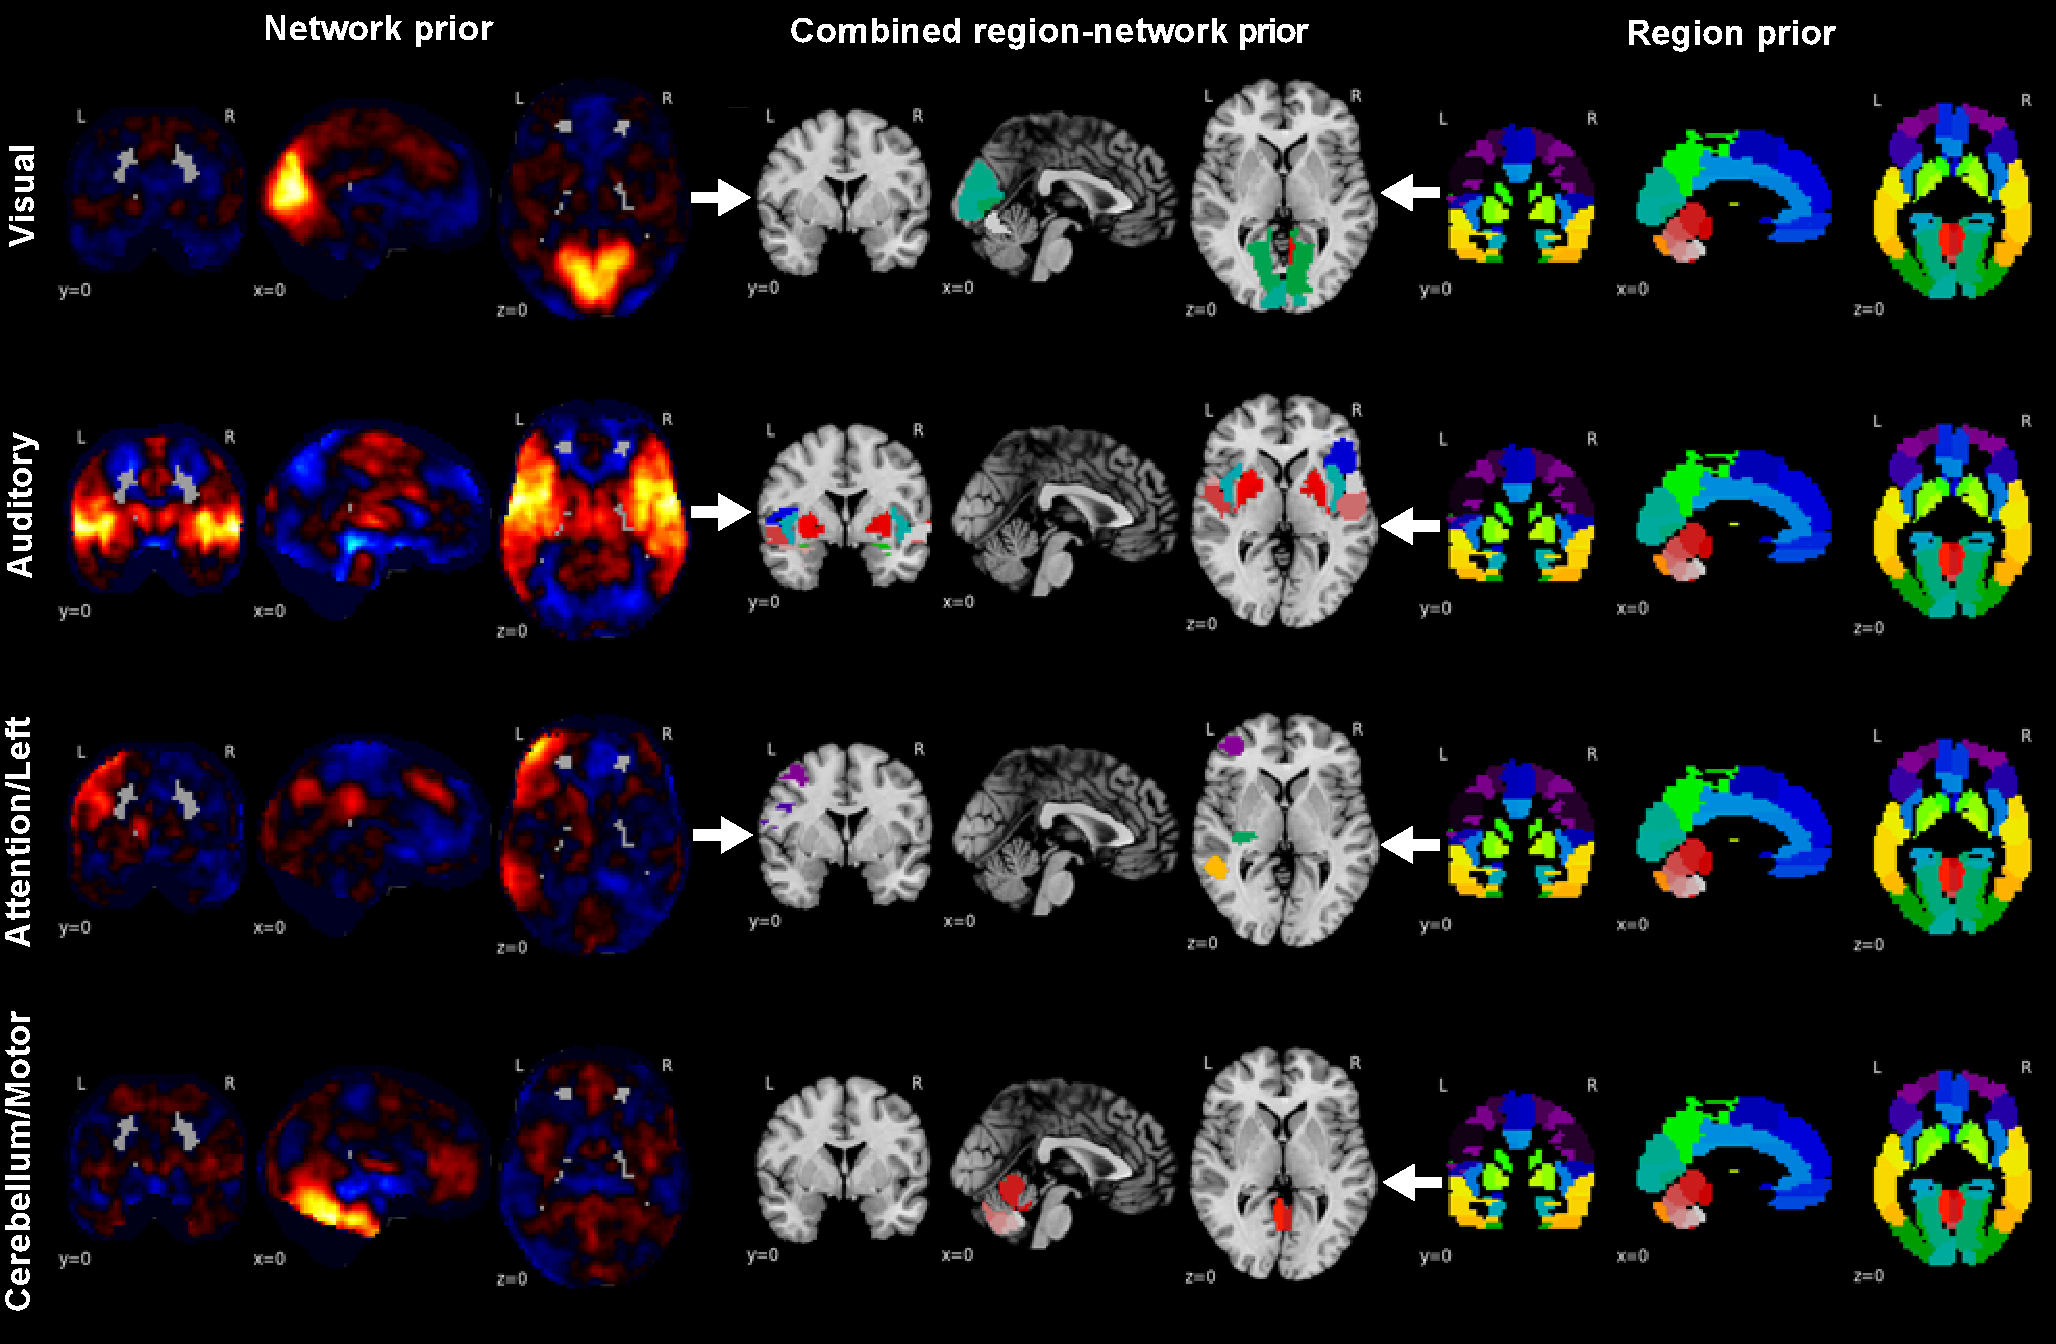
\includegraphics[width=0.8\textwidth]{../figures/reg_net_prior_colin.pdf}
\vspace{-0.2cm}
\caption{\textbf{Building blocks of the region-network tree.}
Neurobiological priors introduced into the classification problem 
by hierarchical structured sparsity are displayed.
\textit{Left:} Continuous, partially overlapping brain network priors
(\textit{hot-colored}, taken from \cite{smith2009})
accommodate the functional integration
perspective of brain organization.
\textit{Right:} Discrete, non-overlapping brain region priors
(\textit{single-colored}, taken from \cite{crad12})
accommodate the functional segregation perspective.
\textit{Middle:} These two types of predefined voxel groups are incorporated
into hierarchical priors of parent networks with their
descending region nodes.
\textit{Top to bottom:} Four examplary region-network priors
are shown, including
the early cortex that processes
visual and sound information from the environment,
a well-known attentional circuit in the left brain hemisphere,
and
the cerebellum that is involved in motor behavior.
}
\label{fig_priors}
\end{figure*}


\begin{figure*}
\begin{centering}
% 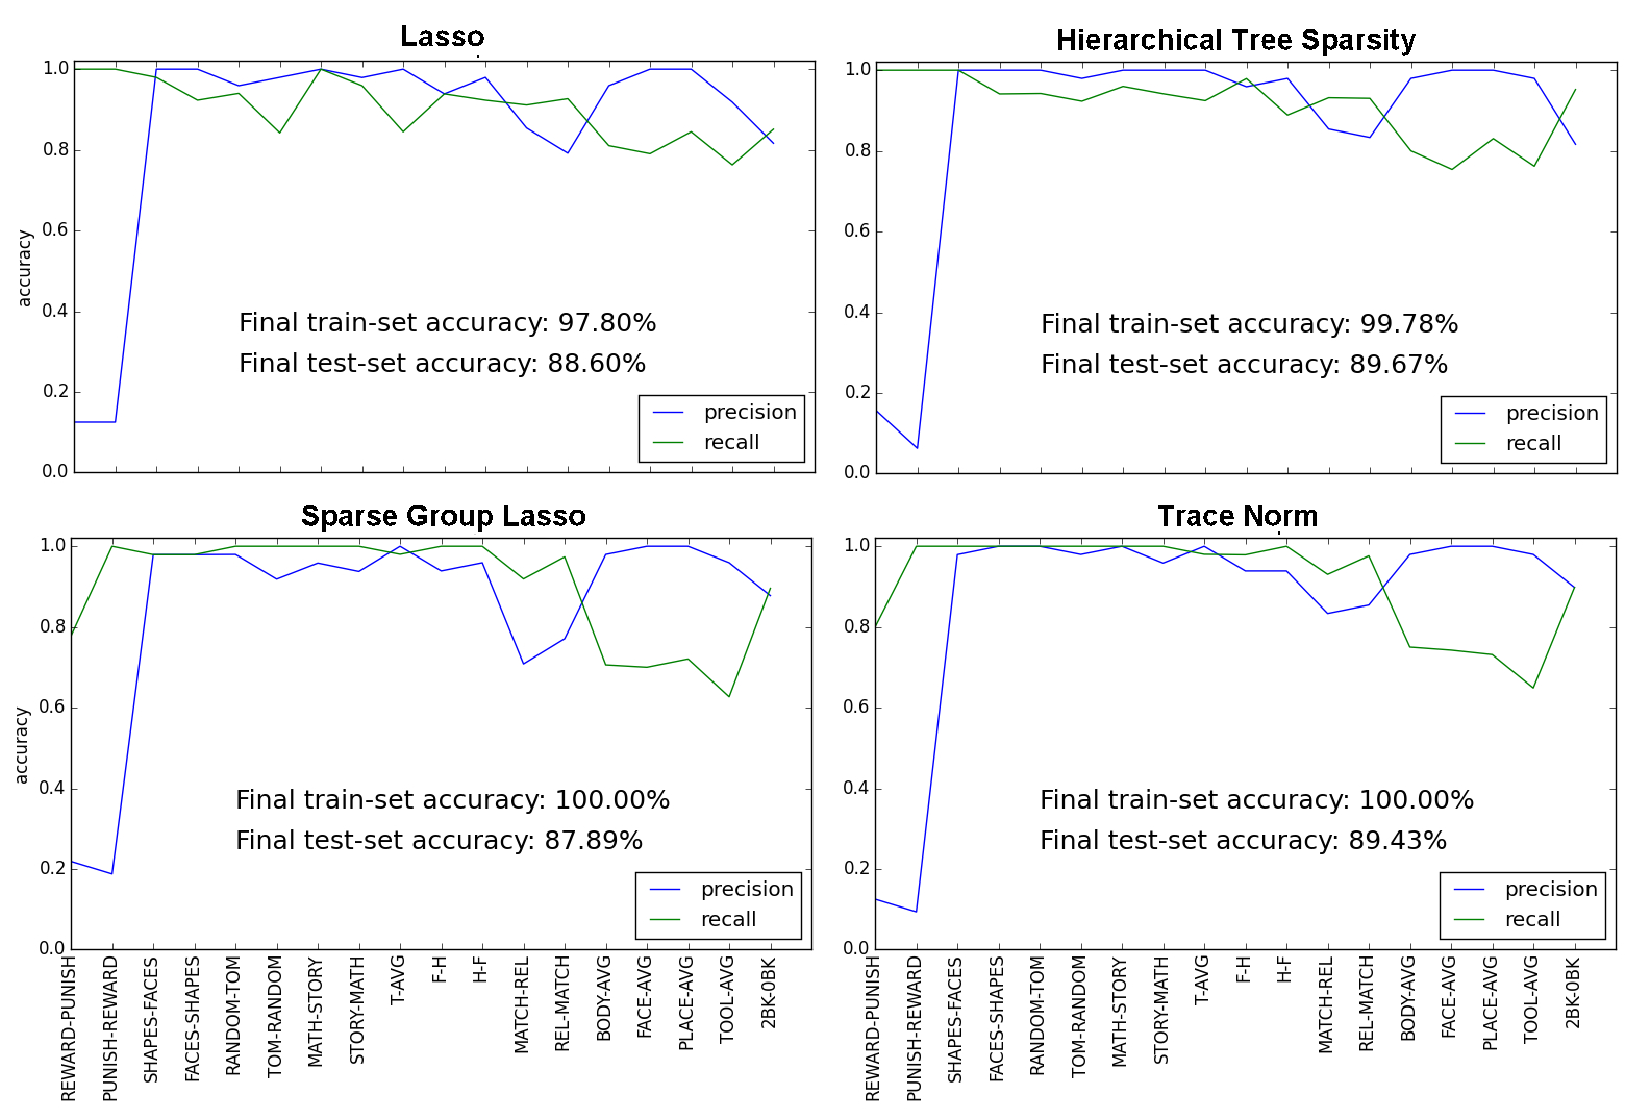
\includegraphics[width=1.00\textwidth]{../figures/sparsities.pdf}
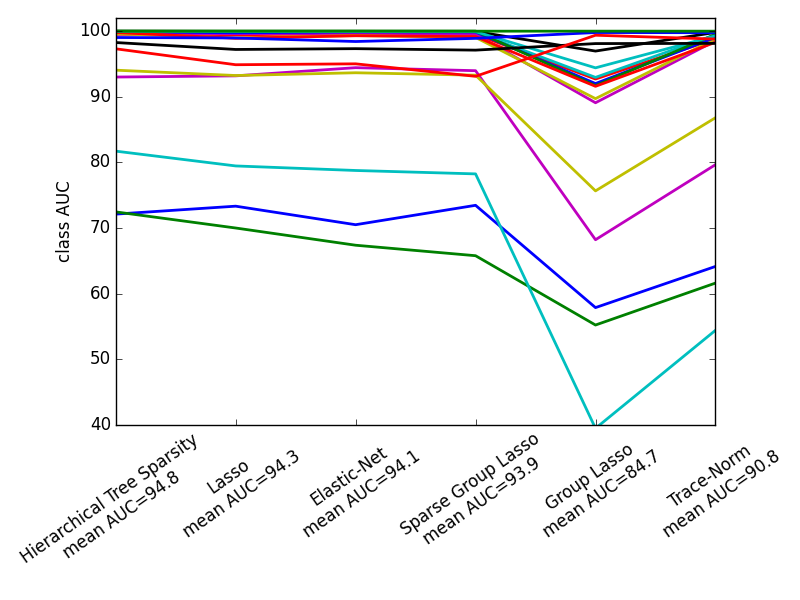
\includegraphics[width=0.55\textwidth]{../figures/ROC_ALL.png}
\vspace{-0.4cm}
\caption{\textbf{Prediction performance across sparsity priors.}
Comparison of the performance of logistic regression estimators
with 6 different structured and unstructered sparsity penalties
in classifying neural activity from 18 psychological tasks.
The class-wise area under the curve (AUC, \textit{colors})
is obtained on an identical test set.
%
\textit{Hierarchical Tree Sparsity}: Structured
$\ell_1/\ell_2$-block-norm with a hierarchy of
both region and network priors
exhibited the best out-of-sample performance
($\alpha = 1, \beta = 1$).
\textit{Lasso}: Unstructured $\ell_1$-penalized logistic regression
imposed a minimum of relevant brain voxels without
assuming special structure.
\textit{Elastic-Net}: Unstructured logistic regression
with interpolation between $\ell_1$- and $\ell_2$-norm 
imposed an equilibrium between sparsity and model fit.
\textit{(Sparse) Group Sparsity}: Structured $\ell_1/\ell_2$-block
norm (with additional $\ell_1$ term)
imposed region compartments, but naive to network structure.
\textit{Trace-norm}: Structured trace-norm penalization
imposed low-rank structure
with sparsity of network patterns, but naive to region structure.
%
A priori knowledge of both region and network neighborhoods
was hence most beneficial for predicting psychological tasks from
brain maps.
}
\end{centering}
\label{fig_sparsities}
\end{figure*}


% \paragraph{Benchmarking hierarchical tree sparsity against
\subsection{Benchmarking hierarchical tree sparsity against
common sparsity penalties}
Hierarchical region-network priors have been systematically
evaluated against other popular choices of sparse classification algorithms
in an 18-class scenario
(Figure \ref{fig_sparsities}).
%
Logistic regression with $\ell_1/\ell_2$ block norm penalization
incorporated a hierarchy of previously known region and network neighborhoods
for a neurobiological bias of the statistical estimation
($\alpha = 1, \beta = 1$).
%
Vanilla logistic regression with $\ell_1$-penalization
does not assume any previously known special structure.
This classification estimator embraces a vision of neural activity structure
that expects a minimum of
topographically and functionally independent brain voxel to be relevant.
%
Logistic regression with (sparse) group sparsity
imposes a structured $\ell_1/\ell_2$ block norm (with additional $\ell_1$ term)
with a known atlas of region voxel groups onto the statistical estimation process.
This supervised estimator shrinks and selects the coefficients
of topographically compact voxel groups expected to be relevant together.
%
Logistic regression with trace-norm penalization
imposed low-rank structure \cite{harchaoui2012large}.
This supervised classification algorithm
expected a minimum of unknown network patterns
to be relevant.
%
% The stratified and shuffled training data were submitted
% to a nested cross-validation scheme
% for model selection and model assessment.
% In the inner CV layer, the logistic regression estimators
% have been trained in a one-versus-rest design that
% distinguishes each class from
% the respective 17 other classes
% (number of maximal iterations=$100$, tolerance=$0.001$).
% In the outer CV layer, grid search
% selected among candidates for the respective $\lambda$ parameter
% by searching between $10^{-2}$ and $10^{1}$ in 9 steps on a logarithmic scale.
% Importantly, the thus selected sparse logistic regression classifier was
% evaluated on an identical test set in all settings.


Across analyses,
hierarchial tree sparsity was most successful
in distinguishing unseen neural activity maps from 18 psychological tasks
(89.7\% multi-class accuracy, mean AUC 94.8 [+/- 9.1 standard deviation]
mean precision 86.7, mean recall 91.5).
It was closely followed by logistic regression
structured by trace-norm regularization
(89.4\%, mean AUC 90.8 [+/- 14.8],
precision 86.4, recall 91.3).
Lasso featured an average performance comparing to the other sparse estimators
(88.60\%, mean AUC 94.3 [+/- 9.3],
precision 85.7, recall 90.3).
Elastic-Net, in turn, featured an
average performance comparing to the other sparse estimators
(88.1\%, mean AUC 94.1 [+/- 10.2],
precision 84.8, recall 84.1).
Introducing a priori knowledge of brain region compartments
by sparse group sparsity
(87.9\%, mean AUC 93.9 [+/- 10.1], precision 84.8, recall 89.5)
and
by group sparsity
(87.9\%, mean AUC 84.7 [+/- 17.3], precision 85.3, recall 90.3)
performed worst.
%
In an important subanalysis,
the gain of the combined region-network prior was also confirmed by
selectively zeroing the $\eta_g$ coefficients of all region groups
or all network groups in the hierarchical prior.
Removing region structure from the prior achieved
88,84\% accuracy,
while removing network structure from the prior achieved
87,05\% accuracy.
These results from partial priors are indeed outperformed
the full region-network tree prior at 89,67\% accuracy.
%
In sum,
biasing sparse model selection by domain knowledge of region-network hierarchies
outcompeted other types of frequently used sparse penalization techniques.



\begin{figure*}
\begin{centering}
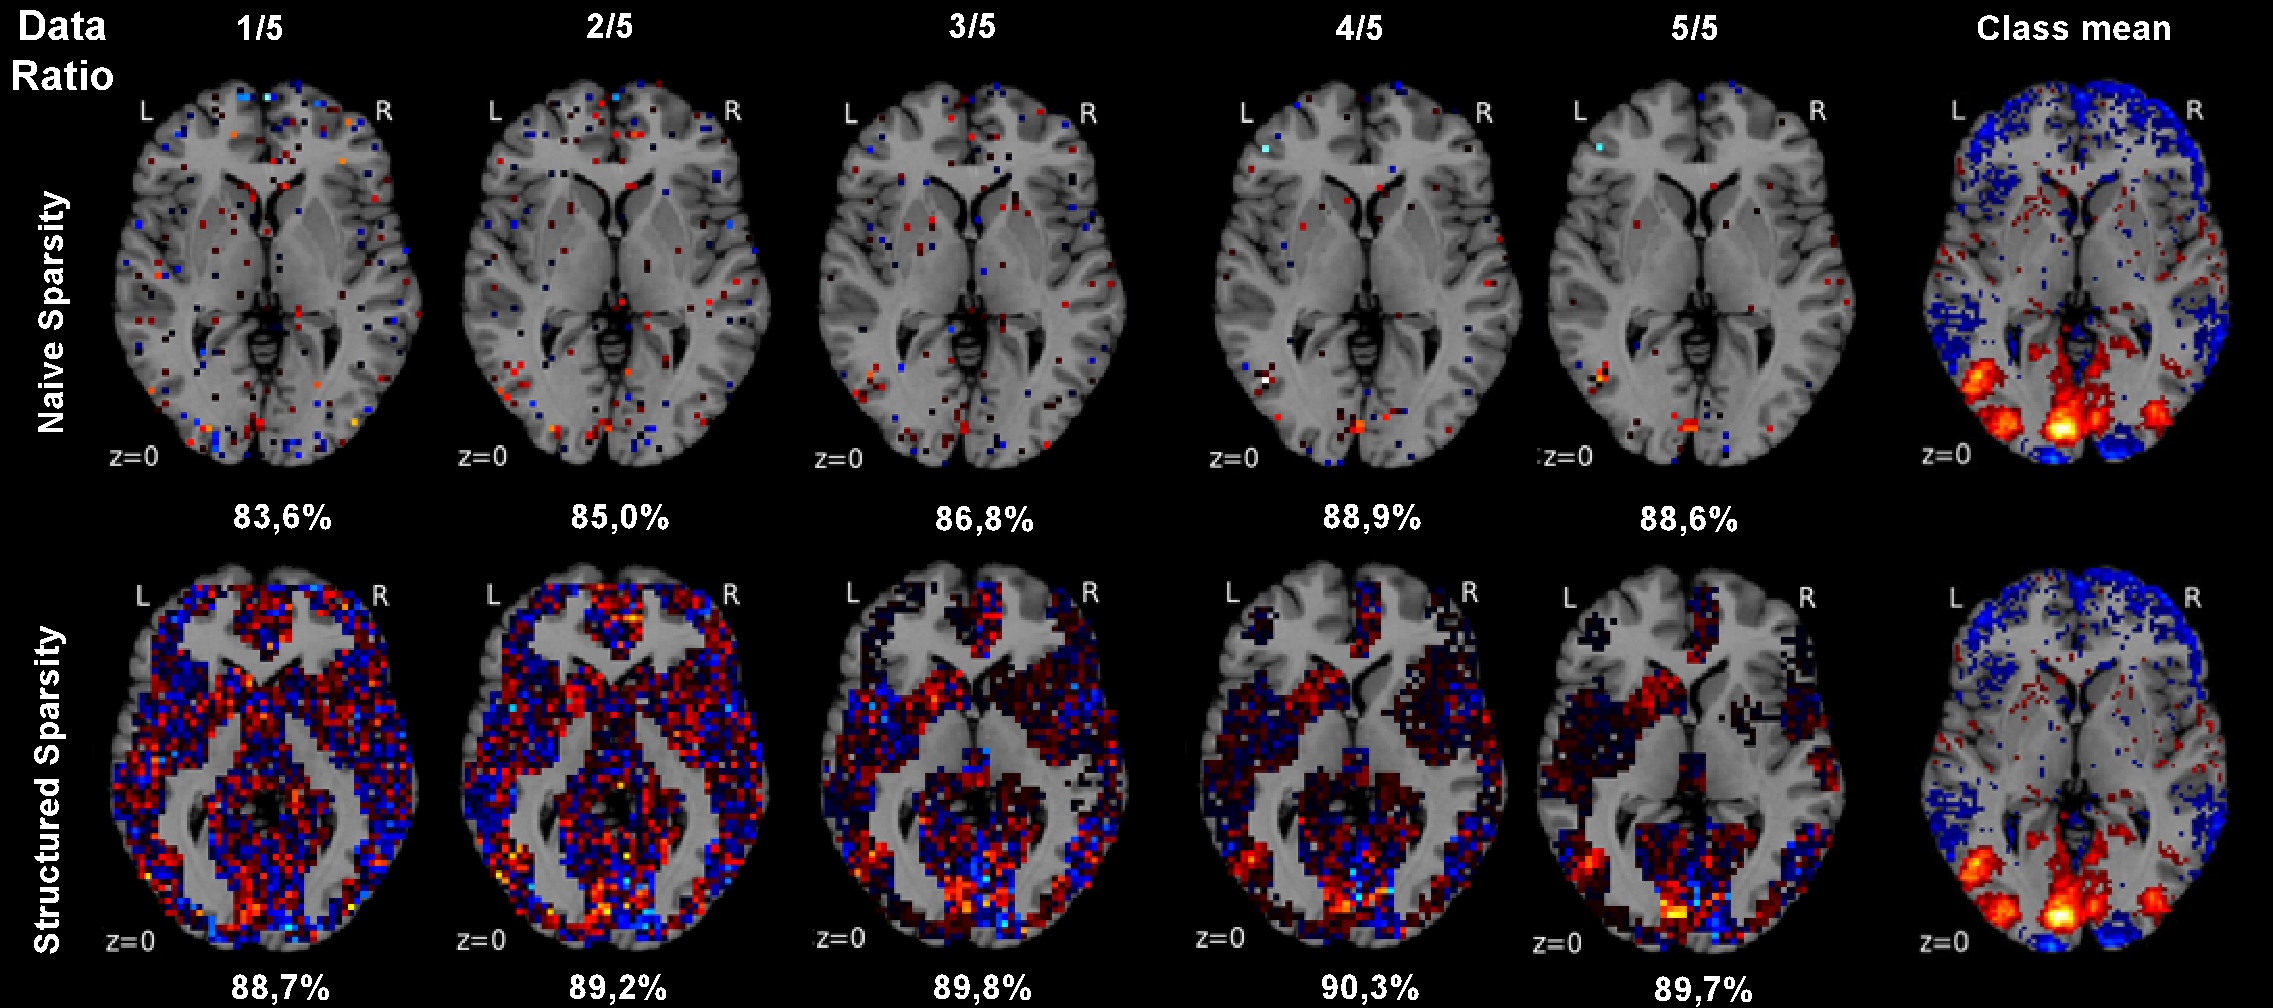
\includegraphics[width=0.80\textwidth]{../figures/dataratio_trans.pdf}
%\vspace{-0.6cm}
\caption{\textbf{Naive versus informed sparse model selection
across training set sizes.}
Ordinary $\ell_1$-penalized logistic regression
(\textit{upper row})
is compared
to hierarchical-tree-penalized logistic regression
($\alpha = 1, \beta = 1$, \textit{lower row})
with increasing fraction
of the available training data (\textit{left to right columns}).
For one example (i.e., ``View tools'') from 18 psychological tasks,
unthresholded axial maps of model weights
are shown for comparison against
the sample average of that class
(\textit{rightmost column}, thresholded at the $75^{th}$ percentile).
The support recovery of that exemplary task is given
as Pearson correlation (cf. methods).
%
In the data-scarce scenario,
typical for brain imaging,
hierarchical tree sparsity achieves much
better support recovery with the biggest difference
in model performance (83.7\% versus 89.0\%).
%
In the data-rich scenario,
neurobiologically informed logistic regression
profits more from the available information quantities than
neurobiologically naive logistic regression.
}
\label{fig_dataratio}
\end{centering}
\end{figure*}



\subsection{Sample complexity of naive versus informed sparse model selection}
% \paragraph{Sample complexity of naive versus informed sparse model selection.}
Subsequently, the sample complexity of
$\ell_1$-penalized and hierarchical-tree-penalized logistic regression
($\alpha = 1, \beta = 1$)
were quantitatively compared (Figure \ref{fig_dataratio}).
Region-network priors should bias model selection towards more
neurobiologically plausible classification estimators.
This should yield better out-of-sample generalization and
support recovery than
neurobiology-naive $\ell_1$-constrained logistic regression
in the data-scarce and data-rich scenarios.
%
The HCP task data with examples from 18
psychological tasks were first divided into
90\% of training set (i.e., 7584 neural activity maps) and
10\% of test set (i.e., 842 neural activity maps).
Both learning algorithms were fitted based on the
training set at different subsampling fractions:
20\% (1516 neural activity maps),
40\% (3033 maps),
60\% (4550 maps),
80\% (6067 maps), and
100\% (7584 maps).

% results: accuracy
Regarding classification performance on the always same test set,
$\ell_1$-penalized versus hierarchical-tree-penalized logistic regression
achieved
83.6\% versus 88.7\% (20\% of training data),
85.0\% versus 89.2\% (40\%),
86.8\% versus 89.8\% (60\%),
88.9\% versus 90.3\% (80\%),
88.6\% versus 89.7\% (100\%) accuracy.
% results: sparsity
Regarding model sparsity,
the measure $s = \frac{||w||_1}{||w||_F}$ was computed from
the model weights $w$ of both penalized estimators
for each of the 18 classes.
The $\ell_1$-penalized logistic regression
yielded the mean (+/- standard deviation) sparsities
50.0 (+/- 2.6), 45.4 (+/- 2.3), 40.0 (+/- 2.4), 30.9 (+/- 2.0), and 24.0 (+/- 2.3)
after model fitting with 20\% to 100\% training data.
The hierarchical-tree-penalized logistic regression
yield the sparsities
163.2 (+/- 0.7), 160.2 (+/- 1.8), 132.1 (+/- 3.3), 116.2 (+/- 4.4), and 88.4 (+/- 8.4)
after fitting 20\% to 100\% of the training data.
% results: support recovery
Finally, the support recovery was quantified by
Pearson correlation $\rho$ between vectors of
the zscored model coefficients
and
the zscored sample maps for each class.
$\ell_1$-penalized versus hierarchical-tree-penalized logistic regression
achieved a mean $\rho$ (+/- standard deviation) recovery of
0.10 (+/- 0.03) versus 0.13 (+/- 0.04),
0.11 (+/- 0.03) versus 0.13 (+/- 0.05),
0.13 (+/- 0.04) versus 0.17 (+/- 0.05),
0.16 (+/- 0.04) versus 0.22 (+/- 0.05), and
0.19 (+/- 0.05) versus 0.29 (+/- 0.06)
based on 20\% to 100\% training data.



Three observations have been made.
In the data-scarce scenario (i.e., 1/5 of available training data),
hierarchical tree sparsity achieved the biggest advantage
in out-of-sample performance by 5,11\% as well as
better support recovery with weight maps already much closer
to the class averages
\cite{varoquaux2012small}.
In the case of scarce training data, which is typical for the brain imaging domain,
regularization by region-network priors thus allowed for
more effective extraction of classification-relevant structure
from the neural activity maps.
%
Across training data fractions,
the weight maps from ordinary logistic regression exhibited
higher variance and more zero coefficients
than hierarchical tree logistic regression.
Given the usually high multicollinearity in neuroimaging data,
this observation is likely to reflect instable selection of
representatives among class-responsive predictor groups
due to the $\ell_1$-norm penalization.
%
In the data-rich scenario (i.e., entire training data used for model fitting),
neurobiologically informed logistic regression
profited more from the increased information quantities than
neurobiologically naive logistic regression.
That is, the region-network priors actually further enhance the similarity
to the weight maps even in abundant input data.
This was the case although
the maximal classification performance of $\approx$90\% has already
been reached with small training data fractions by the structured estimator.
In contrast, 
the unstructured estimator reached this generalization performance
only with bigger input data quantities.
%
\begin{figure*}
\begin{centering}
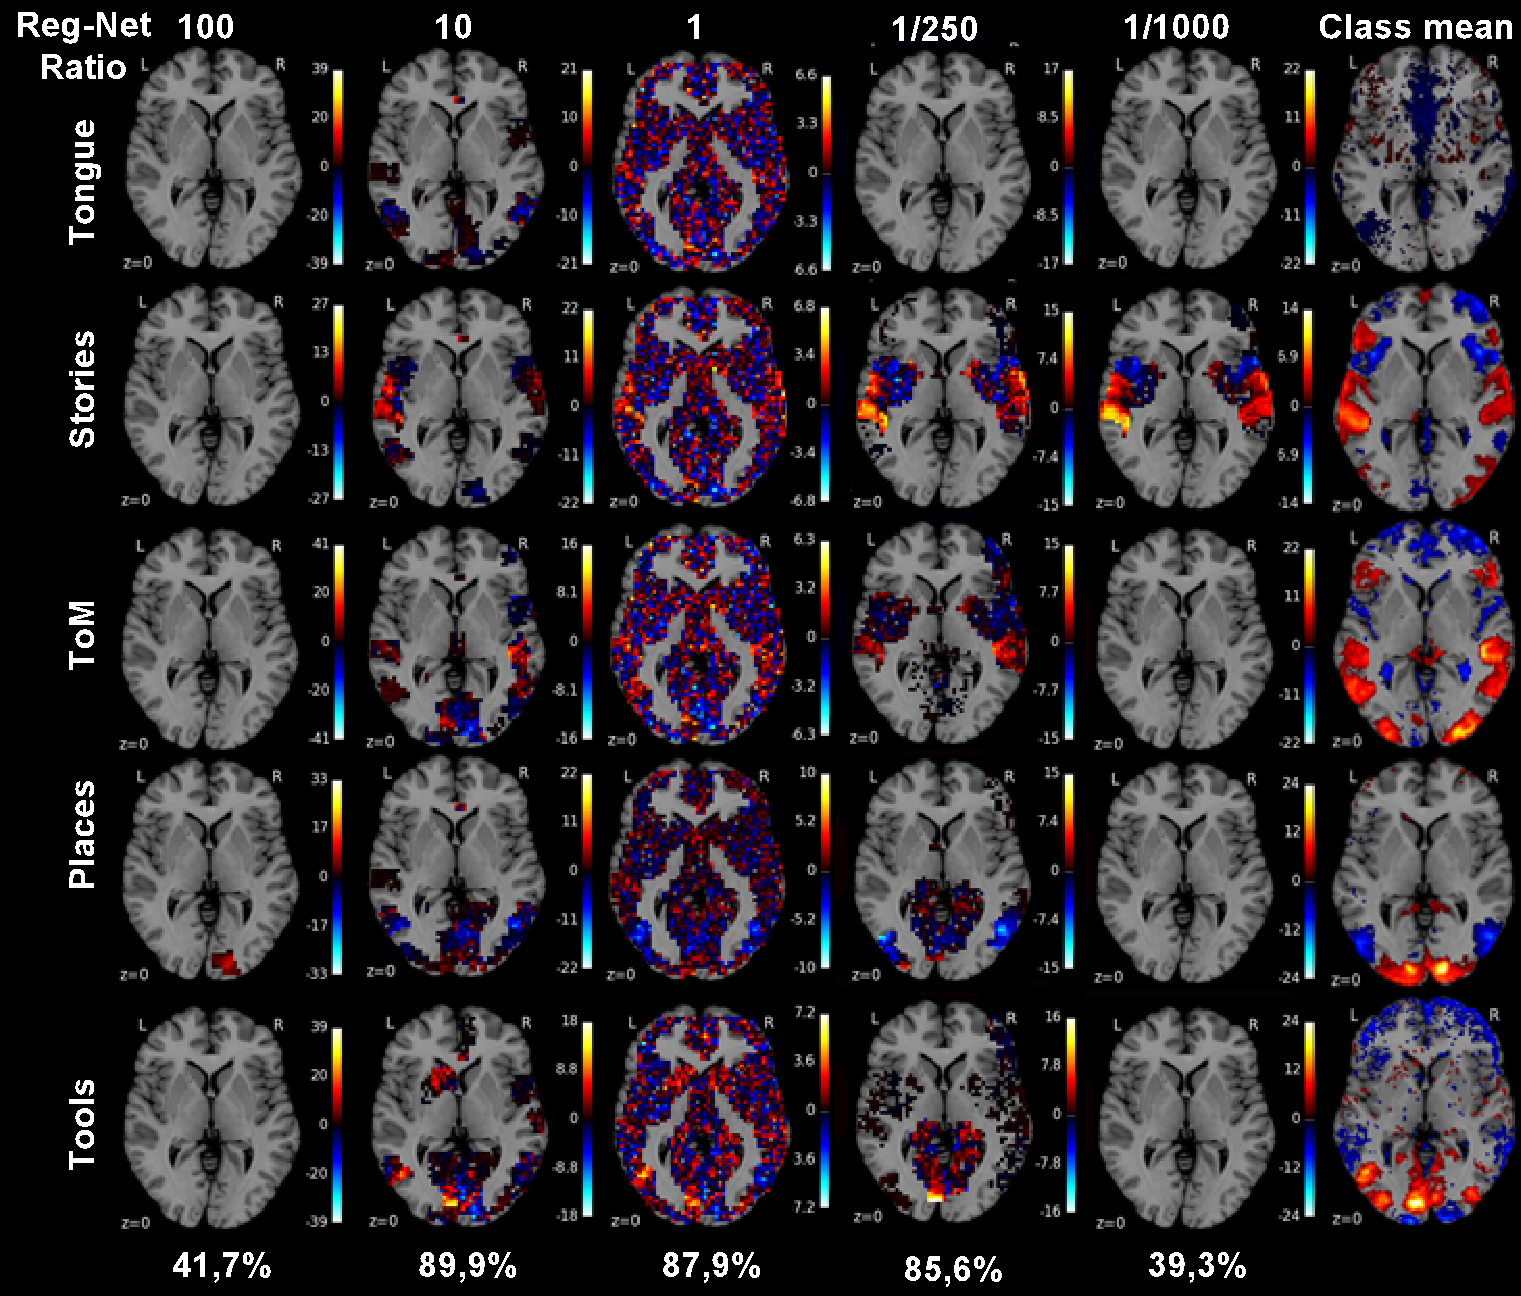
\includegraphics[width=0.90\textwidth]{../figures/reg_net_ratio_colin.pdf}
%\vspace{-0.6cm}
\caption{\textbf{Support recovery as a function of
region and network emphasis.}
The relative impact of the region and network priors
on model selection
is systematically varied against each other
(i.e., $\alpha$ and $\beta$ are changed reciprocally).
This region-network ratio (\textit{upper fractions}) weighted voxel groups
to priviledge sparse models in function space
that acknowledge known brain region neighborhoods
(\textit{left columns}) or
known brain networks neighborhoods
(\textit{right columns}).
Among the 18 classes, the model weights are shown for the psychological
tasks (\textit{from top to bottom}): tongue movement, listening stories,
taking somebody else's perspective (ToM, "theory of mind"),
as well as
viewing locations and tools.
The 18-class out-of-sample accuracy is indicated
on the \textit{bottom} and
the class-wise mean neural activty
(\textit{rightmost column}, thresholded at the $75^{th}$ percentile).
%
Different emphasis on regions versus networks
in hierarchical structured sparsity can
yield comparable model performance.
%
Favoring region versus network structure during model selection
recovers complementary aspects of the neural activity pattern.
%
Equal region and network emphasis yields more dispersed,
less interpretable model choices.
}
\label{fig_regnetratio}
\end{centering}
\end{figure*}
%
\subsection{Support recovery as a function of region-network emphasis}
% \paragraph{Support recovery as a function of region-network emphasis.}
Finally, the relative importance of the
region and network priors within the hierarchical tree prior
was quantified (Figure \ref{fig_regnetratio}).
The group weight $\eta_g$ of region priors was multiplied with a
region-network ratio, while the
group weight $\eta_g$ of network priors was divided by that
region-network ratio. For instance, a region-network ratio of 3
increased the relative importance of known region structure
by multiplying $\beta = \frac{3}{1}$ to
$\eta_g$ of all region group penalties
and multiplying
$\alpha = \frac{1}{3}$ to $\eta_g$ of all network group penalties
(Table \ref{table_reg_net_ratio}).


\begin{table*}[]
\centering
\caption{Out-of-sample performance by region-network emphasis}
\begin{tabular}{l|l|l|l|l|l|l|l|l|l|l|l|l|l|l|l}
\textbf{Reg-Net Ratio} & 500 & 100  & 50   & 10   & 5    & 2    & 1    & $\frac{1}{2}$  & $\frac{1}{5}$  & $\frac{1}{10}$ & $\frac{1}{50}$ & $\frac{1}{100}$ & $\frac{1}{250}$ & $\frac{1}{500}$ & $\frac{1}{1000}$ \\ \hline
\textbf{Accuracy {[}\%{]}}      & 3.8          & 41.7 & 63.7 & 89.9 & 89.9 & 88.5 & 87.9 & 87.9 & 87.9 & 87.8 & 88.6 & 87.8  & 85.6  & 67.2  & 39,3  
\end{tabular}
\label{table_reg_net_ratio}
\end{table*}

As the most important observation,
a range between region-dominant and network-dominant structured penalties
yielded quantitatively almost identical generalization to new data
but qualitatively different decision functions manifested in the weight maps
(Figure \ref{fig_regnetratio}, second and forth column).
Classification models with many zero coefficients but high absolute
coefficients in either region compartments or network compartments
can similarly extrapolate to unseen neural activity maps.
Second,
these achieve classification performance
comparable to equilibrated region-network priors
that set less voxel coefficients to zero and spread the
probability mass with lower absolute coefficients across the whole brain
(Figure \ref{fig_regnetratio}, third column in the middle).
Third,
overly strong emphasis on either level of the hierarchical prior
can yield the neurobiologically informative results with maps
of the most necessary region or network structure for
statistically significant out-of-sample performance
(Figure \ref{fig_regnetratio}, leftmost and rightmost columns).
%
In sum,
stratifying the hierarchical tree penalty between region and network emphasis
suggests that \textit{class-specific region-network weights}
might offer more performant and more interpretable classification models
in the future.



\section{Conclusion}
Relevant structure in neuroimaging data has long been investigated
according to two separate organizational principles:
functional segregation into discrete brain regions
\cite{passingham2002}
and functional integration by interregional brain networks
\cite{sporns14nn}.
Both organizational principles are however inextricable because
a specialized brain region communicates input and output with other regions
and a brain network subserves complex function by
orchestrating its region nodes.
This suggests hierarchical statistical models
as an underexploited opportunity for imaging imaging analysis.
%
This proof-of-concept study demonstrates the simultaneous exploitation of
both these neurobiological compartments
for sparse variable selection and high-dimensional prediction
in a reference dataset.
%
Introducing existing domain knowledge into model selection
allowed privileging members of the function space
that are most neurobiologically plausible.
%
This statistically and neurobiologically desirable bias
is shown to enhance
both model interpretability and generalization performance,
although these statistical-learning goals are typically in conflict.



The present approach has important advantages over previous
analysis strategies that rely on dimensionality reduction of
the neuroimaging data to harness the curse of dimensionality.
They often use preliminary pooling functions within regions
or regression against network templates
for subsequent supervised learning on the aggregated feature space.
Such lossy approaches divided into feature engineering and inference steps
\textit{i)} can only satisfy the specialization or
integration account of brain organization,
\textit{ii)} depend on the ground truth being a region or network effect,
and
\textit{iii)} cannot issue individual coefficients for every brain voxels.
%
Hierarchical region-network sparsity addresses these shortcomings
by estimating individual voxel contributions
while benefitting from their functional segregation and integration
to restrict statistical complexity.
%
Viewed from the bias-variance tradeoff,
our modification to logistic regression estimators
entailed a large decrease in model variance but only a modest
increase in model bias.
Viewed from the Vapnik-Chervonenkis dimensions,
this entailed a healthy decrease in the complexity capacity of the prediction model
with a higher chance of generalizing to unobserved data.



In the future,
region-network sparsity priors could be incorporated into various
pattern-learning methods in systems neuroscience.
%
This includes supervised methods for whole-brain classification and regression
with one or several target variables.
The principled regularization scheme could inform
unsupervised structure-discovery by
matrix factorization and clustering algorithms
\cite{jenatton2009structured, witten2010framework}.
Additionally,
model regularization by hierarchical structured sparsity could be extended
from the spatial domain of neural activity to
priors of coherent spatiotemporal activity structure
\cite{gramfort2011tracking}.
%
The deterministic choice of a region and network atlas
could further be avoided by
sparse selection of overcomplete region-network dictionaries.
Non-hierarchical penalty terms will probably allow for
more complex structured sparsity that
extend the recently enabled parent-children dependencies.
%
Ultimately,
successful high-dimensional inference is
an important prerequisite
for predicting diagnosis,
disease trajectories, and treatment response
in personalized psychiatry and neurology.



% \paragraph{Acknowledgment.}
% {\small The research leading to these results has received funding from the
% European Union Seventh Framework Programme (FP7/2007-2013)
% under grant agreement no. 604102 (Human Brain Project).
% Data were provided by the Human Connectome Project.
% Further support was received from
% the German National Academic Foundation (D.B.),
% the German Research Foundation (BZ2/2-1 and BZ2/3-1 to D.B.),
% and the MetaMRI associated team (B.T., G.V.).
% }

  
\small
% \bibliographystyle{plainnat}
\bibliographystyle{icml2016}
\bibliography{../paper_refs}
% \bibliography{paper_refs}




\end{document} 


% This document was modified from the file originally made available by
% Pat Langley and Andrea Danyluk for ICML-2K. This version was
% created by Lise Getoor and Tobias Scheffer, it was slightly modified  
% from the 2010 version by Thorsten Joachims & Johannes Fuernkranz, 
% slightly modified from the 2009 version by Kiri Wagstaff and 
% Sam Roweis's 2008 version, which is slightly modified from 
% Prasad Tadepalli's 2007 version which is a lightly 
% changed version of the previous year's version by Andrew Moore, 
% which was in turn edited from those of Kristian Kersting and 
% Codrina Lauth. Alex Smola contributed to the algorithmic style files.  
